%%%%%%%%%%%%%%%%%%%%%%%%%%%%%%%%%%%%%%%%%%%%%%%%%%%%%%%%%%%%%%%%%%%%%%%%%%%%%%%
%                                                                             %
% Copyright (C) 2015,2017 Edward d'Auvergne                                   %
%                                                                             %
% This file is part of the program relax (http://www.nmr-relax.com).          %
%                                                                             %
% This program is free software: you can redistribute it and/or modify        %
% it under the terms of the GNU General Public License as published by        %
% the Free Software Foundation, either version 3 of the License, or           %
% (at your option) any later version.                                         %
%                                                                             %
% This program is distributed in the hope that it will be useful,             %
% but WITHOUT ANY WARRANTY; without even the implied warranty of              %
% MERCHANTABILITY or FITNESS FOR A PARTICULAR PURPOSE.  See the               %
% GNU General Public License for more details.                                %
%                                                                             %
% You should have received a copy of the GNU General Public License           %
% along with this program.  If not, see <http://www.gnu.org/licenses/>.       %
%                                                                             %
%%%%%%%%%%%%%%%%%%%%%%%%%%%%%%%%%%%%%%%%%%%%%%%%%%%%%%%%%%%%%%%%%%%%%%%%%%%%%%%


% Frame order theory.
%%%%%%%%%%%%%%%%%%%%%

\section{Frame order theory}




% Frame order introduction.
%~~~~~~~~~~~~~~~~~~~~~~~~~~

\subsection{Frame order introduction}




% The ordering of a vector.
%--------------------------

\subsubsection{The ordering of a vector}

Let $\mu(t)$ be a time dependent vector defined within an arbitrary fixed frame $F$ as
\begin{equation}
    \mu(t) = \left[ \delta_x, \delta_y, \delta_z \right]^T
\end{equation}

where $\delta_i$ is the time dependent direction cosine between the unit vector and the axis $i$ of frame $F$.
Key for understanding the statistical mechanics of a second rank rotational process is the time dependence of the outer product
\begin{align}
    P(t) &= \mu(t) \otimes \mu(t) , \label{eq: time dependent vector outer product} \\
            &= \begin{bmatrix}
                \delta_x^2       & \delta_x\delta_y & \delta_x\delta_z \\
                \delta_y\delta_x & \delta_y^2       & \delta_y\delta_z \\
                \delta_z\delta_x & \delta_z\delta_y & \delta_z^2
               \end{bmatrix} .
\end{align}

Assuming statistical mechanical ensemble averaging, the observable expected value of the matrix $P(t)$ is a matrix which defines the ordering of the vector $\mu(t)$ within the frame $F$.
This order matrix is
\begin{subequations}
\begin{align}
    S(t) 
        &\equiv \overline{P(t)} , \\
        &= \overline{\mu(t) \otimes \mu(t)} , \label{eq: order matrix expected outer product} \\
        &= \overline{\begin{bmatrix}
                \delta_x^2       & \delta_x\delta_y & \delta_x\delta_z \\
                \delta_y\delta_x & \delta_y^2       & \delta_y\delta_z \\
                \delta_z\delta_x & \delta_z\delta_y & \delta_z^2
        \end{bmatrix}} , \label{eq: order matrix direction cosine} \\
        &= \begin{bmatrix}
            S_{xx}(t) & S_{xy}(t) & S_{xz}(t) \\
            S_{yx}(t) & S_{yy}(t) & S_{yz}(t) \\
            S_{zx}(t) & S_{zy}(t) & S_{zz}(t)
        \end{bmatrix} , \label{eq: order matrix}
\end{align}
\end{subequations}

where
\begin{equation}
    S_{ij}(t) = \overline{\delta_i \delta_j} .
\end{equation}

Because of the symmetry $S_{ij}(t) = S_{ji}(t)$, the order matrix has 6 unique elements.

Assuming that the time dependent process modulating $\mu(t)$ is much faster than the evolution period $t_{\textrm{max}}$ of the observed physical interaction, for example the weak molecular alignment process which induces residual dipolar couplings (RDCs) and pseudo-contact shifts (PCSs) in NMR, the order matrix which gives rise to the non-isotropic effect is equation~\ref{eq: order matrix direction cosine} at $t_{\textrm{max}} = \infty$.
Hence the non-zero order matrix is
\begin{equation}
    S(\infty) = \begin{bmatrix}
                S_{xx}(\infty) & S_{xy}(\infty) & S_{xz}(\infty) \\
                S_{yx}(\infty) & S_{yy}(\infty) & S_{yz}(\infty) \\
                S_{zx}(\infty) & S_{zy}(\infty) & S_{zz}(\infty)
              \end{bmatrix} .
\end{equation}




% The ordering of a frame.
%--------------------------

\subsubsection{The ordering of a frame}

Let the frame $C(t)$ be time dependent within an arbitrary fixed frame $F$.
After a time period $t$ the shift from $C(0)$ to $C(t)$ is given by the rotation
\begin{equation}
    R(t) = \begin{bmatrix}
               c_{xx} & c_{xy} & c_{xz} \\
               c_{yx} & c_{yy} & c_{yz} \\
               c_{zx} & c_{zy} & c_{zz}
           \end{bmatrix}
         \equiv \begin{bmatrix}
               \delta_{xx} & \delta_{xy} & \delta_{xz} \\
               \delta_{yx} & \delta_{yy} & \delta_{yz} \\
               \delta_{zx} & \delta_{zy} & \delta_{zz}
           \end{bmatrix} ,
\end{equation}

where rotation matrix element $c_{ij}$ is equivalent to the direction cosine $\delta_{ij}$ between axis $i$ of $C(t)$ and axis $j$ of $C(0)$.
For second rank physical processes modulated by rotational motions, analogously to the outer product expected value of~\ref{eq: order matrix expected outer product}, the time dependence of the process is governed by the outer product
\begin{equation} \label{eq: 2nd degree frame order definition}
    \FOtwo(t) = \overline{R(t) \otimes R(t)}
\end{equation}

This is a rank-4, three dimensional rotational tensor defining the ordering of the frame $C(t)$ after a period $t$ within the original frame $C(0)$.
This is the definition of the second degree frame order tensor.

The matrix form of the second degree frame order tensor in rank-2, 9D Kronecker product notation is
\begin{equation} \label{eq: frame order matrix 9D}
    \FOtwo(t) =
        \overline{\left[
            \begin{array}{@{}ccc;{2pt/4pt}ccc;{2pt/4pt}ccc@{}}
                \delta_{xx}^2          & \delta_{xx}\delta_{xy} & \delta_{xx}\delta_{xz} & \delta_{xy}\delta_{xx} & \delta_{xy}^2          & \delta_{xy}\delta_{xz} & \delta_{xz}\delta_{xx} & \delta_{xz}\delta_{xy} & \delta_{xz}^2          \\
                \delta_{xx}\delta_{yx} & \delta_{xx}\delta_{yy} & \delta_{xx}\delta_{yz} & \delta_{xy}\delta_{yx} & \delta_{xy}\delta_{yy} & \delta_{xy}\delta_{yz} & \delta_{xz}\delta_{yx} & \delta_{xz}\delta_{yy} & \delta_{xz}\delta_{yz} \\
                \delta_{xx}\delta_{zx} & \delta_{xx}\delta_{zy} & \delta_{xx}\delta_{zz} & \delta_{xy}\delta_{zx} & \delta_{xy}\delta_{zy} & \delta_{xy}\delta_{zz} & \delta_{xz}\delta_{zx} & \delta_{xz}\delta_{zy} & \delta_{xz}\delta_{zz} \\ \hdashline[2pt/4pt]
                \delta_{yx}\delta_{xx} & \delta_{yx}\delta_{xy} & \delta_{yx}\delta_{xz} & \delta_{yy}\delta_{xx} & \delta_{yy}\delta_{xy} & \delta_{yy}\delta_{xz} & \delta_{yz}\delta_{xx} & \delta_{yz}\delta_{xy} & \delta_{yz}\delta_{xz} \\
                \delta_{yx}^2          & \delta_{yx}\delta_{yy} & \delta_{yx}\delta_{yz} & \delta_{yy}\delta_{yx} & \delta_{yy}^2          & \delta_{yy}\delta_{yz} & \delta_{yz}\delta_{yx} & \delta_{yz}\delta_{yy} & \delta_{yz}^2          \\
                \delta_{yx}\delta_{zx} & \delta_{yx}\delta_{zy} & \delta_{yx}\delta_{zz} & \delta_{yy}\delta_{zx} & \delta_{yy}\delta_{zy} & \delta_{yy}\delta_{zz} & \delta_{yz}\delta_{zx} & \delta_{yz}\delta_{zy} & \delta_{yz}\delta_{zz} \\ \hdashline[2pt/4pt]
                \delta_{zx}\delta_{xx} & \delta_{zx}\delta_{xy} & \delta_{zx}\delta_{xz} & \delta_{zy}\delta_{xx} & \delta_{zy}\delta_{xy} & \delta_{zy}\delta_{xz} & \delta_{zz}\delta_{xx} & \delta_{zz}\delta_{xy} & \delta_{zz}\delta_{xz} \\
                \delta_{zx}\delta_{yx} & \delta_{zx}\delta_{yy} & \delta_{zx}\delta_{yz} & \delta_{zy}\delta_{yx} & \delta_{zy}\delta_{yy} & \delta_{zy}\delta_{yz} & \delta_{zz}\delta_{yx} & \delta_{zz}\delta_{yy} & \delta_{zz}\delta_{yz} \\
                \delta_{zx}^2          & \delta_{zx}\delta_{zy} & \delta_{zx}\delta_{zz} & \delta_{zy}\delta_{zx} & \delta_{zy}^2          & \delta_{zy}\delta_{zz} & \delta_{zz}\delta_{zx} & \delta_{zz}\delta_{zy} & \delta_{zz}^2
            \end{array}
        \right]} ,
\end{equation}

where
\begin{equation}
    \overline{\delta_{ij}\delta_{kl}} \equiv \overline{c_{ij}c_{kl}} .
\end{equation}


This is a rank-2, 3D order matrix of rank-2, 3D order matrices.
To see this, the $T_{14}$ rank-4 matrix transpose of $\FOtwo$ in Kronecker product notation is
\begin{equation} \label{eq: frame order matrix 9D T14}
    \FO^{T_{14}}(t) =
        \overline{\left[
            \begin{array}{@{}ccc;{2pt/4pt}ccc;{2pt/4pt}ccc@{}}
                \delta_{xx}^2          & \delta_{yx}\delta_{xx} & \delta_{zx}\delta_{xx} & \delta_{xy}\delta_{xx} & \delta_{yy}\delta_{xx} & \delta_{zy}\delta_{xx} & \delta_{xz}\delta_{xx} & \delta_{yz}\delta_{xx} & \delta_{zz}\delta_{xx} \\
                \delta_{xx}\delta_{yx} & \delta_{yx}^2          & \delta_{zx}\delta_{yx} & \delta_{xy}\delta_{yx} & \delta_{yy}\delta_{yx} & \delta_{zy}\delta_{yx} & \delta_{xz}\delta_{yx} & \delta_{yz}\delta_{yx} & \delta_{zz}\delta_{yx} \\
                \delta_{xx}\delta_{zx} & \delta_{yx}\delta_{zx} & \delta_{zx}^2          & \delta_{xy}\delta_{zx} & \delta_{yy}\delta_{zx} & \delta_{zy}\delta_{zx} & \delta_{xz}\delta_{zx} & \delta_{yz}\delta_{zx} & \delta_{zz}\delta_{zx} \\ \hdashline[2pt/4pt]
                \delta_{xx}\delta_{xy} & \delta_{yx}\delta_{xy} & \delta_{zx}\delta_{xy} & \delta_{xy}^2          & \delta_{yy}\delta_{xy} & \delta_{zy}\delta_{xy} & \delta_{xz}\delta_{xy} & \delta_{yz}\delta_{xy} & \delta_{zz}\delta_{xy} \\
                \delta_{xx}\delta_{yy} & \delta_{yx}\delta_{yy} & \delta_{zx}\delta_{yy} & \delta_{xy}\delta_{yy} & \delta_{yy}^2          & \delta_{zy}\delta_{yy} & \delta_{xz}\delta_{yy} & \delta_{yz}\delta_{yy} & \delta_{zz}\delta_{yy} \\
                \delta_{xx}\delta_{zy} & \delta_{yx}\delta_{zy} & \delta_{zx}\delta_{zy} & \delta_{xy}\delta_{zy} & \delta_{yy}\delta_{zy} & \delta_{zy}^2          & \delta_{xz}\delta_{zy} & \delta_{yz}\delta_{zy} & \delta_{zz}\delta_{zy} \\ \hdashline[2pt/4pt]
                \delta_{xx}\delta_{xz} & \delta_{yx}\delta_{xz} & \delta_{zx}\delta_{xz} & \delta_{xy}\delta_{xz} & \delta_{yy}\delta_{xz} & \delta_{zy}\delta_{xz} & \delta_{xz}^2          & \delta_{yz}\delta_{xz} & \delta_{zz}\delta_{xz} \\
                \delta_{xx}\delta_{yz} & \delta_{yx}\delta_{yz} & \delta_{zx}\delta_{yz} & \delta_{xy}\delta_{yz} & \delta_{yy}\delta_{yz} & \delta_{zy}\delta_{yz} & \delta_{xz}\delta_{yz} & \delta_{yz}^2          & \delta_{zz}\delta_{yz} \\
                \delta_{xx}\delta_{zz} & \delta_{yx}\delta_{zz} & \delta_{zx}\delta_{zz} & \delta_{xy}\delta_{zz} & \delta_{yy}\delta_{zz} & \delta_{zy}\delta_{zz} & \delta_{xz}\delta_{zz} & \delta_{yz}\delta_{zz} & \delta_{zz}^2
            \end{array}
        \right]} .
\end{equation}


The 3D matrix in the top left corner is the ordering of the x-axis with itself, the central matrix is the ordering of the y-axis with itself, and the bottom right is the ordering of the z-axis with itself.
The off-diagonal 3D matrices are the cross-correlations between the three axes.
Using the notation $e_x$, $e_y$ and $e_z$ for the orthogonal axis system of the time dependent frame $C(t)$, the second degree frame order matrix can be written as
\begin{equation}
    \FO^{T_{14}}(t) =
        \begin{bmatrix}
            \overline{e_x \otimes e_x} & \overline{e_x \otimes e_y} & \overline{e_x \otimes e_z} \\
            \overline{e_y \otimes e_x} & \overline{e_y \otimes e_y} & \overline{e_y \otimes e_z} \\
            \overline{e_z \otimes e_x} & \overline{e_z \otimes e_y} & \overline{e_z \otimes e_z}
        \end{bmatrix} .
\end{equation}

If the rank-2, 3D order matrix between the axes A and B is denoted as
\begin{equation}
    S_{\textrm{AB}}(t) = \overline{e_A \otimes e_B},
\end{equation}

then the frame order matrix is
\begin{equation}
    \FO^{T_{14}}(t) =
        \begin{bmatrix}
            S_{\textrm{XX}}(t) & S_{\textrm{XY}}(t) & S_{\textrm{XZ}}(t) \\
            S_{\textrm{YX}}(t) & S_{\textrm{YY}}(t) & S_{\textrm{YZ}}(t) \\
            S_{\textrm{ZX}}(t) & S_{\textrm{ZY}}(t) & S_{\textrm{ZZ}}(t)
        \end{bmatrix} .
\end{equation}


The frame order matrix is diagonally symmetric, as can be seen in the $T_{14}$ transpose of the matrix in rank-2, 9D Kronecker product form (equation~\ref{eq: frame order matrix 9D T14}, hence for the second degree frame order matrix there are 45 unique elements.
For the 9D Kronecker product notation of equation~\ref{eq: frame order matrix 9D}, this transformed diagonal symmetry can be schematically represented as

\setlength{\unitlength}{0.5cm}
\begin{picture}(19,9)
    % Frame order symbol.
    \put(6.5,4.0){$\FOtwo(t) = $}

    % Brackets.
    \put(10.0,0.0){\line(0,1){9}}
    \put(10.0,0.0){\line(1,0){0.2}}
    \put(10.0,9.0){\line(1,0){0.2}}
    \put(19.0,0.0){\line(0,1){9}}
    \put(19.0,0.0){\line(-1,0){0.2}}
    \put(19.0,9.0){\line(-1,0){0.2}}

    % Full stop.
    \put(19.5,4.0){.}

    % Elements.
    \multiput(10.5,0.5)(0,1){9}{\circle*{0.1}}
    \multiput(11.5,0.5)(0,1){9}{\circle*{0.1}}
    \multiput(12.5,0.5)(0,1){9}{\circle*{0.1}}
    \multiput(13.5,0.5)(0,1){9}{\circle*{0.1}}
    \multiput(14.5,0.5)(0,1){9}{\circle*{0.1}}
    \multiput(15.5,0.5)(0,1){9}{\circle*{0.1}}
    \multiput(16.5,0.5)(0,1){9}{\circle*{0.1}}
    \multiput(17.5,0.5)(0,1){9}{\circle*{0.1}}
    \multiput(18.5,0.5)(0,1){9}{\circle*{0.1}}

    % All symmetry lines in red.
    \color{Red}

    % 1st column.
    %\put(10.5,0.35){\line(1,1){8}}  <c_ij^2> != <c_ji^2>.
    \put(10.4,1.5){\line(0,1){2}}
    \put(10.6,2.5){\line(0,1){4}}
    %\put(10.5,4.5){\line(1,1){4}}  <c_ij^2> != <c_ji^2>.
    \put(10.4,5.5){\line(0,1){2}}

    % 2nd column.
    \put(11.5,0.6){\line(1,0){2}}
    \put(11.5,1.6){\line(1,1){2}}
    \put(11.5,2.5){\line(1,2){2}}
    \put(11.5,3.5){\line(1,-1){2}}
    \put(11.5,4.6){\line(1,0){2}}
    \put(11.5,5.5){\line(1,1){2}}
    \put(11.5,6.5){\line(1,-2){2}}
    \put(11.5,7.6){\line(1,-1){2}}
    \put(11.5,8.6){\line(1,0){2}}

    % 3rd column.
    \put(12.5,0.4){\line(1,0){4}}
    \put(12.5,1.5){\line(2,1){4}}
    \put(12.5,2.4){\line(1,1){4}}
    \put(12.5,3.5){\line(2,-1){4}}
    \put(12.5,4.4){\line(1,0){4}}
    \put(12.5,5.5){\line(2,1){4}}
    \put(12.5,6.4){\line(1,-1){4}}
    \put(12.5,7.5){\line(2,-1){4}}
    \put(12.5,8.4){\line(1,0){4}}

    % 5th column.
    %\put(14.5,0.4){\line(1,1){4}}  <c_ij^2> != <c_ji^2>.
    \put(14.4,1.5){\line(0,1){2}}
    \put(14.6,2.5){\line(0,1){4}}
    \put(14.4,5.5){\line(0,1){2}}

    % 6th column.
    \put(15.5,0.6){\line(1,0){2}}
    \put(15.5,1.5){\line(1,1){2}}
    \put(15.5,2.5){\line(1,2){2}}
    \put(15.5,3.6){\line(1,-1){2}}
    \put(15.5,4.6){\line(1,0){2}}
    \put(15.5,5.6){\line(1,1){2}}
    \put(15.5,6.5){\line(1,-2){2}}
    \put(15.5,7.5){\line(1,-1){2}}
    \put(15.5,8.6){\line(1,0){2}}

    % 9th column.
    \put(18.4,1.5){\line(0,1){2}}
    \put(18.6,2.5){\line(0,1){4}}
    \put(18.4,5.5){\line(0,1){2}}

\end{picture}

When rotational symmetries are present in the time modulation of the frame $C(t)$ then, according to \citet{Perrin36}, the averages of the double products $\overline{c_{ij}c_{kl}}$ where an index appears only once is zero.
In this case, the active frame order matrix elements are
\begin{equation} \label{eq: frame order matrix 9D symmetry}
    \FOtwo(t) =
        \left[
            \begin{array}{@{}ccc;{2pt/4pt}ccc;{2pt/4pt}ccc@{}}
                \overline{\delta_{xx}^2}     & .                                 & .                                 & .                                 & \overline{\delta_{xy}^2}     & .                                 & .                                 & .                                 & \overline{\delta_{xz}^2}    \\
                .                            & \overline{\delta_{xx}\delta_{yy}} & .                                 & \overline{\delta_{xy}\delta_{yx}} & .                            & .                                 & .                                 & .                                 & .                           \\
                .                            & .                                 & \overline{\delta_{xx}\delta_{zz}} & .                                 & .                            & .                                 & \overline{\delta_{xz}\delta_{zx}} & .                                 & .                           \\ \hdashline[2pt/4pt]
                .                            & \overline{\delta_{yx}\delta_{xy}} & .                                 & \overline{\delta_{yy}\delta_{xx}} & .                            & .                                 & .                                 & .                                 & .                           \\
                \overline{\delta_{yx}^2}     & .                                 & .                                 & .                                 & \overline{\delta_{yy}^2}     & .                                 & .                                 & .                                 & \overline{\delta_{yz}^2}    \\
                .                            & .                                 & .                                 & .                                 & .                            & \overline{\delta_{yy}\delta_{zz}} & .                                 & \overline{\delta_{yz}\delta_{zy}} & .                           \\ \hdashline[2pt/4pt]
                .                            & .                                 & \overline{\delta_{zx}\delta_{xz}} & .                                 & .                            & .                                 & \overline{\delta_{zz}\delta_{xx}} & .                                 & .                           \\
                .                            & .                                 & .                                 & .                                 & .                            & \overline{\delta_{zy}\delta_{yz}} & .                                 & \overline{\delta_{zz}\delta_{yy}} & .                           \\
                \overline{\delta_{zx}^2}     & .                                 & .                                 & .                                 & \overline{\delta_{zy}^2}     & .                                 & .                                 & .                                 & \overline{\delta_{zz}^2}
            \end{array}
        \right] .
\end{equation}

This matrix consists of 15 unique elements.
It is the weighted sum of the three rank-4 identity matrices $I_1$, $I_2$ and $I_3$.




% The fourth rank identity matrices.
%-----------------------------------

\subsubsection{The fourth rank identity matrices}

According to \citet{Spencer80}, the rank-4 identity matrices are defined as
\begin{subequations}
\begin{align}
    I_1 &= \delta_{ij} \delta_{kl} e_i \otimes e_j \otimes e_k \otimes e_l , \label{eq: rank-4 identity matrix 1} \\
    I_2 &= \delta_{ik} \delta_{jl} e_i \otimes e_j \otimes e_k \otimes e_l , \label{eq: rank-4 identity matrix 2} \\
    I_3 &= \delta_{il} \delta_{kj} e_i \otimes e_j \otimes e_k \otimes e_l , \label{eq: rank-4 identity matrix 3}
\end{align}
\end{subequations}

where $\delta_{ij}$ is the Kronecker delta and $e_i$ are the axes.
In general, the identity matrix is
\begin{equation}
    I = \left( \lambda \delta_{ij} \delta_{kl} + \mu \delta_{ik} \delta_{jl} + \nu \delta_{il} \delta_{kj} \right) e_i \otimes e_j \otimes e_k \otimes e_l . \\
\end{equation}

Expanding~\ref{eq: rank-4 identity matrix 1} to~\ref{eq: rank-4 identity matrix 3} to 9D Kronecker product matrix form,
\begin{subequations}
\begin{align}
    I_1 &=
        \left[
            \begin{array}{*{9}{@{}>{\centering\arraybackslash}p{2em}@{}}}
                1 & . & . & . & 1 & . & . & . & 1 \\
                . & . & . & . & . & . & . & . & . \\
                . & . & . & . & . & . & . & . & . \\
                . & . & . & . & . & . & . & . & . \\
                1 & . & . & . & 1 & . & . & . & 1 \\
                . & . & . & . & . & . & . & . & . \\
                . & . & . & . & . & . & . & . & . \\
                . & . & . & . & . & . & . & . & . \\
                1 & . & . & . & 1 & . & . & . & 1
            \end{array}
        \right], \\
    I_2 &=
        \left[
            \begin{array}{*{9}{@{}>{\centering\arraybackslash}p{2em}@{}}}
                1 & . & . & . & . & . & . & . & . \\
                . & 1 & . & . & . & . & . & . & . \\
                . & . & 1 & . & . & . & . & . & . \\
                . & . & . & 1 & . & . & . & . & . \\
                . & . & . & . & 1 & . & . & . & . \\
                . & . & . & . & . & 1 & . & . & . \\
                . & . & . & . & . & . & 1 & . & . \\
                . & . & . & . & . & . & . & 1 & . \\
                . & . & . & . & . & . & . & . & 1
            \end{array}
        \right] , \\
    I_3 &=
        \left[
            \begin{array}{*{9}{@{}>{\centering\arraybackslash}p{2em}@{}}}
                1 & . & . & . & . & . & . & . & . \\
                . & . & . & 1 & . & . & . & . & . \\
                . & . & . & . & . & . & 1 & . & . \\
                . & 1 & . & . & . & . & . & . & . \\
                . & . & . & . & 1 & . & . & . & . \\
                . & . & . & . & . & . & . & 1 & . \\
                . & . & 1 & . & . & . & . & . & . \\
                . & . & . & . & . & 1 & . & . & . \\
                . & . & . & . & . & . & . & . & 1
            \end{array}
        \right] .
\end{align}
\end{subequations}

The identity matrices are related to each other via the rank-4 matrix transposes
\begin{subequations}
\begin{align}
    I_2 &= I_1^{T_{14}} = I_1^{T_{23}} , \\
    I_3 &= I_1^{T_{24}} = I_1^{T_{13}} .
\end{align}
\end{subequations}

In the case of unrestricted motions, the time limits of the frame order matrix are
\begin{equation}
    \FOtwo(t = 0) = I_1 ,
\end{equation}

and
\begin{equation}
    \FOtwo(t = \infty) = \tfrac{1}{3} I_2 .
\end{equation}




% Tensor power of the frame order.
%---------------------------------

\subsubsection{Tensor power of the frame order}

The rank-4, 3D frame order tensor of equation~\ref{eq: 2nd degree frame order definition} on page~\pageref{eq: 2nd degree frame order definition} was derived for second order rotational physical processes.
However this can be generalised for physical processes of all orders.
The tensor power of the time dependent rotation matrix $R(t)$ is defined as
\begin{equation}
    R^{\otimes n}(t) \overset{\mathrm{def}}{=} R(t) \otimes \cdots \otimes R(t) ,
\end{equation}

where the outer product is repeated $n$ times.
Therefore let the frame order tensor be defined as
\begin{equation} \label{eq: frame order definition}
    \FOn(t) = \overline{R^{\otimes n}(t)} ,
\end{equation}

where $n$ is the order of the physical process.
The rank of the 3D tensors is $2n$.
The first few frame order tensors of rank-2, rank-4, rank-6, and rank-8 are
\begin{subequations}
\begin{align}
    \FOone(t) &= \overline{R(t)} , \\
    \FOtwo(t) &= \overline{R(t) \otimes R(t)} , \\
    \FOthree(t) &= \overline{R(t) \otimes R(t) \otimes R(t)} , \\
    \FOfour(t) &= \overline{R(t) \otimes R(t) \otimes R(t) \otimes R(t)} .
\end{align}
\end{subequations}

In index and direction cosine notation,
\begin{subequations}
\begin{align}
    &\FOone_{ij}(t) = \overline{\delta_{ij}} , \\
    &\FOtwo_{ijkl}(t) = \overline{\delta_{ij}\delta_{kl}} , \\
    &\FOthree_{ijklmn}(t) = \overline{\delta_{ij}\delta_{kl}\delta_{mn}} , \\
    &\FOfour_{ijklmnop}(t) = \overline{\delta_{ij}\delta_{kl}\delta_{mn}\delta_{op}} .
\end{align}
\end{subequations}




% The frame order motional eigenframe.
%-------------------------------------

\subsubsection{The frame order motional eigenframe}

The rotation matrices of the general frame order tensor of equation~\ref{eq: frame order definition} can be decomposed into a time dependent and time independent component.
The original frame $F$ can be defined as the motional eigenframe of the system and a new arbitrary frame $F'$ introduced.
The forward rotation from the reference frame $F'$ to the motional eigenframe $F$ will be denoted as $R_{\textrm{eigen}}$.
The rotation matrix decomposition is
\begin{equation}
    R'(t) = R_{\textrm{eigen}} \cdot R(t) \cdot R_{\textrm{eigen}}^T .
\end{equation}

Hence the second degree frame order tensor is
\begin{equation}
    \FOtwo = \overline{R'(t) \otimes R'(t)} ,
\end{equation}

Using the mixed product property
\begin{equation}
    AC \otimes BD = (A \otimes B)(C \otimes D) ,
\end{equation}

the arbitrary frame, second degree frame order matrix is
\begin{subequations}
\begin{align}
    \FOtwo &= \overline{\left( R_{\textrm{eigen}} \cdot R(t) \cdot R_{\textrm{eigen}}^T \right) \otimes \left( R_{\textrm{eigen}} \cdot R(t) \cdot R_{\textrm{eigen}}^T \right)} , \\
%           &= \overline{R \cdot \left( R(t) \cdot R^T \right) \otimes R \cdot \left( R(t) \cdot R^T \right)} , \\
           &= \overline{\left(R_{\textrm{eigen}} \otimes R_{\textrm{eigen}} \right) \cdot \left( R(t) \cdot R_{\textrm{eigen}}^T \right) \otimes \left( R(t) \cdot R_{\textrm{eigen}}^T \right)} , \\
           &= \overline{\left(R_{\textrm{eigen}} \otimes R_{\textrm{eigen}} \right) \cdot \left( R(t) \otimes R(t) \right) \cdot \left( R_{\textrm{eigen}}^T \otimes R_{\textrm{eigen}}^T \right)} , \\
           &= \left(R_{\textrm{eigen}} \otimes R_{\textrm{eigen}} \right) \cdot \overline{\left( R(t) \otimes R(t) \right)} \cdot \left( R_{\textrm{eigen}}^T \otimes R_{\textrm{eigen}}^T \right) .
\end{align}
\end{subequations}

Generalising from the \nth{2} to the n$^{\textrm{th}}$-order, the generalised frame order tensor rotation is
\begin{equation} \label{eq: frame order equation, arbitrary frame}
    \FOn(t) = R_{\textrm{eigen}}^{\otimes n} \cdot \overline{R^{\otimes n}(t)} \cdot R_{\textrm{eigen}}^{T \otimes n} .
\end{equation}




% Rotation to the average position frame of the rigid body.
%----------------------------------------------------------

\subsubsection{Rotation to the average position frame of the rigid body}

For the modelling aspect of the frame order theory, one more rotation is required.
In equation~\ref{eq: frame order equation, arbitrary frame}, it is assumed that the starting position for the moving rigid body is that of its motional average.
However in the initial 3D structure, this is not the case and an additional rotation to the average position $R_{\textrm{ave}}$ is required.
Taking this into account, the generalised frame order tensor is defined as
\begin{equation}
    \FOn(t) = R_{\textrm{eigen}}^{\otimes n} \cdot \overline{R^{\otimes n}(t)} \cdot R_{\textrm{eigen}}^{T \otimes n} \cdot R_{\textrm{ave}}^{T \otimes n} ,
\end{equation}

where $R_{\textrm{eigen}}$ is the eigenframe rotation matrix, $R(t)$ is the time dependent rotation matrix, $R_{\textrm{ave}}$ is the rotation from the average domain position to the motional eigenframe, and $\otimes n$ is the n$^{\textrm{th}}$ tensor power.
In applications to physical processes which require numerical integration, pre-rotating the rigid body by $R_{\textrm{ave}}$ to the average position is equivalent but more numerically efficient.
Therefore the $R_{\textrm{ave}}$ can be dropped and equation~\ref{eq: frame order equation, arbitrary frame} used instead.

%For the RDC and PCS which are time independent,
%\begin{equation}
%    R^{\otimes n}(t) = R^{\otimes n}(\infty) .
%\end{equation}
%
%For a single state $i$, its rotation is defined as
%\begin{equation}
%    R_i = R_{\textrm{eigen}} \cdot R(\infty) \cdot R_{\textrm{eigen}}^T \cdot R_{\textrm{ave}}^T .
%\end{equation}
%
%or in a different notation as
%\begin{equation}
%    R_i = R_{\textrm{eigen}} \cdot R_i' \cdot R_{\textrm{eigen}}^T \cdot R_{\textrm{ave}}^T ,
%\end{equation}
%
%where $R_{\textrm{eigen}}$ is the rotation from the average position frame to the motional eigenframe.




% Frame order and the alignment tensor.
%~~~~~~~~~~~~~~~~~~~~~~~~~~~~~~~~~~~~~~

\subsection{Frame order and the alignment tensor}




% The RDC and PCS.
%-----------------

\subsubsection{The RDC and PCS}

For the residual dipolar coupling (RDC) and pseudo-contact shift (PCS) NMR phenomena, both effects are governed by the partial molecular alignment tensor $A$.
For a two domain molecular system, when one domain is internally aligned with for example a paramagnetic lanthanide ion within a magnetic field, the other domain experiences a reduced alignment $\overline{A}$ due to the interdomain motions.


% The RDC.
\paragraph{The RDC}

The residual dipolar coupling is given by
\begin{equation} \label{eq: RDC equation}
    D = d \; \unitvectr^T \cdot A \cdot \unitvectr ,
\end{equation}

where $\unitvectr$ is the internuclear unit vector, $d$ is the dipolar constant defined as
\begin{equation} \label{eq: RDC dipolar constant}
    d = - \frac{3}{2\pi} \frac{\mu_0}{4\pi} \frac{\gamma_I \gamma_S \hbar}{\langle r \rangle^3} ,
\end{equation}

$\mu_0$ is the permeability of free space, $\gamma_i$ is the gyromagnetic ratio of the nucleus $i$, $\hbar$ is Planck's constant divided by $2\pi$, $\langle r \rangle$ is the time averaged internuclear distance, the factor of $\tfrac{1}{2\pi}$ is to convert the constant from radians per second to Hertz, and the factor of three is associated with the alignment tensor.
In the presence of an alignment tensor reduction, and assuming that the fast vibrational and librational internal motions of the vector are statistically self-decoupled from the rigid body motions, the RDC is simply
\begin{equation} \label{eq: reduced RDC equation}
    D = d \; \unitvectr^T \cdot \overline{A} \cdot \unitvectr ,
\end{equation}

as the vector $\unitvectr$ is considered time independent in the molecular reference frame.


% The PCS.
\paragraph{The PCS}

The pseudo-contact shift equation is simply
\begin{subequations} \label{eq: PCS equation}
\begin{align}
    \delta &= \frac{\mu_0}{4\pi} \frac{15 k T}{B_0^2} \frac{1}{\left| \vectr \right|^5} \; \unitvectr^T \cdot A \cdot \unitvectr , \\
           &= \frac{c}{\left| \vectr \right|^5} \; \unitvectr^T \cdot A \cdot \unitvectr , \\
           &= \frac{1}{4\pi} \frac{1}{\left| \vectr \right|^5} \; \unitvectr^T \cdot \chi \cdot \unitvectr ,
\end{align}
\end{subequations}

where $A$ is the alignment tensor, $\chi$ is the magnetic susceptibility tensor, $\unitvectr$ is the lanthanide to nuclear unit vector, and $c$ is the PCS constant defined as
\begin{equation} \label{eq: PCS constant}
    c = \frac{\mu_0}{4\pi} \frac{15 k T}{B_0^2} .
\end{equation}

The alignment tensor reduction process is complicated by the inverse $\left| \vectr \right|^5$ normalisation factor, as $\vectr$ is not time independent in the molecular reference frame.




% Alignment tensor reduction.
%----------------------------

\subsubsection{Alignment tensor reduction}

The statistical mechanics behind the alignment tensor reduction can be expressed as
\begin{equation}
    \overline A = \left\langle \int_0^{\tmax} R^{-1}(\Omega_t) \cdot A \cdot R(\Omega_t) \diff t \right\rangle , \\
\end{equation}

where the angular brackets denote the ensemble averaging, the time integration is for a single molecule over the evolution period of the physical interaction, $\Omega_t$ are the SO(3) rotational angles describing the change in position of the moving rigid body, and $A$ is the full alignment tensor.
Here the alignment tensor has been created by an averaging of the partially restricted Brownian diffusion process of the non-moving component, again both over the ensemble and time, as
\begin{equation}
    A = \left\langle \int_0^{\tmax} R^{-1}(\Omega_t) \cdot F \cdot R(\Omega_t) \diff t \right\rangle , \\
\end{equation}

where $F$ is the molecular frame.
It is assumed that the alignment process of the non-moving domain and the motions of the moving domain are decoupled.

Using the ergodic hypothesis, the averaging process which generates the reduced alignment tensor can be simplified as
\begin{subequations}
\begin{align}
    \overline A &= \overline{R^{-1} \cdot A \cdot R} , \\
                &= \overline{R^T \cdot A \cdot R} .
\end{align}
\end{subequations}

The index notation for a tensor rotation is
\begin{equation}
    T_{ij}' = \sum_{kl} R_{ki} R_{lj} T_{kl} .
\end{equation}

Therefore the reduced alignment tensor in index notation is
\begin{align}
    \overline{A_{ij}}
        &= \sum_{kl} \overline{c_{ki}c_{lj}} A_{kl} , \\
        &= \sum_{kl} \FOtwo_{kilj} A_{kl} ,
\end{align}

where $\FOtwo$ is a rank-4, 3D orientational tensor which will be called the frame order tensor.

Expanding the sum,
\begin{align} \label{eq: alignment tensor reduction, index notation}
    \overline{A_{ij}} & = \FO_{xixj} A_{xx} + \FO_{xiyj} A_{xy} + \FO_{xizj} A_{xz} \nonumber \\
                      & + \FO_{yixj} A_{yx} + \FO_{yiyj} A_{yy} + \FO_{yizj} A_{yz} \nonumber \\
                      & + \FO_{zixj} A_{zx} + \FO_{ziyj} A_{zy} + \FO_{zizj} A_{zz} .
\end{align}

As
\begin{subequations}
\begin{gather}
    A_{ij} = A_{ji} , \\
    A_{zz} = - A_{xx} - A_{yy} ,
\end{gather}
\end{subequations}

equation \ref{eq: alignment tensor reduction, index notation} becomes
\begin{align}
    \overline{A_{ij}} & = \left( \FO_{xixj} - \FO_{zizj} \right) A_{xx}  +  \left( \FO_{yiyj} - \FO_{zizj} \right) A_{yy} \nonumber \\
                      & + \left( \FO_{xiyj} + \FO_{yixj} \right) A_{xy}  +  \left( \FO_{xizj} + \FO_{zixj} \right) A_{xz}  +  \left( \FO_{yizj} + \FO_{ziyj} \right) A_{yz} .
\end{align}

A single element of the reduced tensor is simply a linear combination of all elements of the original tensor multiplied by constants consisting of different combinations of frame order matrix components.

Converting from the rank-2, 3D, symmetric and traceless space of alignment tensors to the rank-1, 5D space, a non-linear frame order superoperator can be written as
\begin{equation} \label{eq: frame order superoperator}
    \overline A = \FOtwo_{\textrm{5D}} \cdot A .
\end{equation}

In matrix notation, this is
\begin{equation} \label{eq: frame order superoperator matrix}
\begin{footnotesize}
    \overline{
        \begin{bmatrix}
            A_{xx} \\
            A_{yy} \\
            A_{xy} \\
            A_{xz} \\
            A_{yz}
        \end{bmatrix}
    } =
        \begin{bmatrix}
            \FO_{xxxx} - \FO_{zxzx}  &  \FO_{yxyx} - \FO_{zxzx} &  \FO_{xxyx} + \FO_{yxxx} &  \FO_{xxzx} + \FO_{zxxx} &  \FO_{yxzx} + \FO_{zxyx} \\
            \FO_{xyxy} - \FO_{zyzy}  &  \FO_{yyyy} - \FO_{zyzy} &  \FO_{xyyy} + \FO_{yyxy} &  \FO_{xyzy} + \FO_{zyxy} &  \FO_{yyzy} + \FO_{zyyy} \\
            \FO_{xxxy} - \FO_{zxzy}  &  \FO_{yxyy} - \FO_{zxzy} &  \FO_{xxyy} + \FO_{yxxy} &  \FO_{xxzy} + \FO_{zxxy} &  \FO_{yxzy} + \FO_{zxyy} \\
            \FO_{xxxz} - \FO_{zxzz}  &  \FO_{yxyz} - \FO_{zxzz} &  \FO_{xxyz} + \FO_{yxxz} &  \FO_{xxzz} + \FO_{zxxz} &  \FO_{yxzz} + \FO_{zxyz} \\
            \FO_{xyxz} - \FO_{zyzz}  &  \FO_{yyyz} - \FO_{zyzz} &  \FO_{xyyz} + \FO_{yyxz} &  \FO_{xyzz} + \FO_{zyxz} &  \FO_{yyzz} + \FO_{zyyz}
        \end{bmatrix}
        \cdot
        \begin{bmatrix}
            A_{xx} \\
            A_{yy} \\
            A_{xy} \\
            A_{xz} \\
            A_{yz}
        \end{bmatrix}
    .
\end{footnotesize}
\end{equation}

Let
\begin{equation}
    \left\{ A_0, A_1, A_2, A_3, A_4 \right\} = \left\{ A_{xx}, A_{yy}, A_{xy}, A_{xz}, A_{yz} \right\} ,
\end{equation}

and assuming the rank-2, 9D Kronecker product form of $\FOtwo_{ij}$ using numerical indices where $\{i,j\} = 0, 1, \dots, 8$, then
\begin{equation}
    \overline{
        \begin{bmatrix}
            A_0 \\
            A_1 \\
            A_2 \\
            A_3 \\
            A_4
        \end{bmatrix}
    } =
        \begin{bmatrix}
            \FO_{00} - \FO_{80}  &  \FO_{40} - \FO_{80} &  \FO_{10} + \FO_{30} &  \FO_{20} + \FO_{60} &  \FO_{50} + \FO_{70} \\
            \FO_{04} - \FO_{84}  &  \FO_{44} - \FO_{84} &  \FO_{14} + \FO_{34} &  \FO_{24} + \FO_{64} &  \FO_{54} + \FO_{74} \\
            \FO_{01} - \FO_{81}  &  \FO_{41} - \FO_{81} &  \FO_{11} + \FO_{31} &  \FO_{21} + \FO_{61} &  \FO_{51} + \FO_{71} \\
            \FO_{02} - \FO_{82}  &  \FO_{42} - \FO_{82} &  \FO_{12} + \FO_{32} &  \FO_{22} + \FO_{62} &  \FO_{52} + \FO_{72} \\
            \FO_{05} - \FO_{85}  &  \FO_{45} - \FO_{85} &  \FO_{15} + \FO_{35} &  \FO_{25} + \FO_{65} &  \FO_{55} + \FO_{75}
        \end{bmatrix}
        \cdot
        \begin{bmatrix}
            A_0 \\
            A_1 \\
            A_2 \\
            A_3 \\
            A_4
        \end{bmatrix}
    .
\end{equation}

For the alignment tensor, the 81 elements of the frame order matrix have recombined into 25 unique scaling factors.



% The alignment tensor is the anisotropic part of a frame order matrix.
%~~~~~~~~~~~~~~~~~~~~~~~~~~~~~~~~~~~~~~~~~~~~~~~~~~~~~~~~~~~~~~~~~~~~~~

\subsubsection{The alignment tensor is the anisotropic part of a frame order matrix}

The alignment tensor is related to the orientational probability tensor by
\begin{equation}
    A = P - \tfrac{1}{3} I .
\end{equation}

The $P$ probability tensor is the average orientation position of the molecule, hence is the average molecular frame $\overline{F}$.
As this frame is simply the rotation matrix relative to the laboratory frame, then
\begin{subequations}
\begin{align}
    P &= \overline{F} , \\
      &= \overline{R} , \\
      &= \FOone .
\end{align}
\end{subequations}

Therefore the alignment tensor can then be written as the anisotropic part of the first degree frame order matrix
\begin{equation}
    A = \FOone - \tfrac{1}{3} I .
\end{equation}




% Single pivoted motions.
%~~~~~~~~~~~~~~~~~~~~~~~~

\subsection{Single pivoted motions}



% Ball-and-socket joint.
%-----------------------

\subsubsection{Atomic level mechanics of the single pivot}

For the PCS, the lanthanide ion to nuclear vector is
\begin{equation}
    \vectr = p_{\textrm{N}} - p_{\textrm{Ln}^{3+}},
\end{equation}

where $p_{\textrm{N}}$ is the Cartesian coordinates of the nucleus of interest and $p_{\textrm{Ln}^{3+}}$ is the position of the aligning lanthanide ion.
$\vectr$ is defined in the alignment frame, and $p_{\textrm{Ln}^{3+}}$ is constant in this frame.
After a forward rotation to the discrete state $i$, the new atomic position in the reference frame is
\begin{equation}
    p_{\textrm{N}}' = R_i \cdot \left( p_{\textrm{N}} - p_{\textrm{P}} \right) + p_{\textrm{P}}.
\end{equation}

where $p_{\textrm{P}}$ is the pivot point of the rotation.
Hence the transformed vector is
\begin{subequations}
\begin{align}
    \vectr_i &= p_{\textrm{N}}^i - p_{\textrm{Ln}^{3+}} , \\
             &= R_i \cdot \left( p_{\textrm{N}} - p_{\textrm{P}} \right) + p_{\textrm{P}} - p_{\textrm{Ln}^{3+}} . \label{eq: pivoted rotation vector i}
\end{align}
\end{subequations}

The set of three vectors are defining this pivoted system are
\begin{subequations}
\begin{align}
    & \vectr_{\textrm{LN}} = p_{\textrm{N}} - p_{\textrm{Ln}^{3+}} , \\
    & \vectr_{\textrm{PN}} = p_{\textrm{N}} - p_{\textrm{P}} , \\
    & \vectr_{\textrm{LP}} = p_{\textrm{P}} - p_{\textrm{Ln}^{3+}} .
\end{align}
\end{subequations}

Let the pre-rotation vectors be
\begin{subequations}
\begin{align}
    & \vectr_{\textrm{LN}}^{(0)} = \vectr_{\textrm{LP}}^{(0)} + \vectr_{\textrm{P} \textrm{N}}^{(0)} , \\
    & \vectr_{\textrm{PN}}^{(0)} , \\
    & \vectr_{\textrm{LP}}^{(0)} .
\end{align}
\end{subequations}

The post-rotation vectors are
\begin{subequations}
\begin{align}
    & \vectr_{\textrm{LN}}^{(1)} = \vectr_{\textrm{LP}}^{(0)} + R_i^{(1)} \cdot \vectr_{\textrm{P} \textrm{N}}^{(0)} , \\
    & \vectr_{\textrm{PN}}^{(1)} = R_i^{(1)} \cdot \vectr_{\textrm{P} \textrm{N}}^{(0)}, \\
    & \vectr_{\textrm{LP}}^{(1)} = \vectr_{\textrm{LP}}^{(0)}.
\end{align}
\end{subequations}

The vector $\vectr_{\textrm{PN}}$ is independent of alignment so can be calculated once per atom, and $\vectr_{\textrm{LP}}$ is independent of alignment and atom position so can be calculate once.




% Pivoted PCS.
%-------------

\subsubsection{PCS and single pivoted motions}

For a single state $i$, the PCS value when substituting~\ref{eq: pivoted rotation vector i} into~\ref{eq: PCS equation} is
\begin{equation}
    \delta = \frac{c}{\left| \vectr_i \right|^5} \; \vectr_i^T \cdot A \cdot \vectr_i . \label{eq: PCS single pivot} \\
\end{equation}

Expanding for the single motion of the lanthanide-atom vector $\vectr_{\textrm{LN}}^{(1)}$, this becomes
\begin{subequations}
\begin{align}
    \delta &= \frac{c}{\left| \vectr_{\textrm{LN}}^{(1)} \right|^5} \;
                    \vectr_{\textrm{LN}}^{(1)^T} \cdot A \cdot \vectr_{\textrm{LN}}^{(1)} , \\
    \delta &= \frac{c}{\left| \vectr_{\textrm{LN}}^{(1)} \right|^5} \;
                    \left( \vectr_{\textrm{LP}}^{(0)} + R_i^{(1)} \cdot \vectr_{\textrm{PN}}^{(0)} \right)^T
                    \cdot A \cdot
                    \left( \vectr_{\textrm{LP}}^{(0)} + R_i^{(1)} \cdot \vectr_{\textrm{PN}}^{(0)} \right) , \\
    \delta &= \frac{c}{\left| \vectr_{\textrm{LN}}^{(1)} \right|^5} \;
                    \left( \vectr_{\textrm{LP}}^{(0)^T} + \vectr_{\textrm{PN}}^{(0)^T} \cdot R_i^{(1)^T} \right)
                    \cdot A \cdot
                    \left( \vectr_{\textrm{LP}}^{(0)} + R_i^{(1)} \cdot \vectr_{\textrm{PN}}^{(0)} \right) , \\
    \delta &= \frac{c}{\left| \vectr_{\textrm{LN}}^{(1)} \right|^5} \; \Bigg[
                    \vectr_{\textrm{PN}}^{(0)^T} \cdot R_i^{(1)^T} \cdot A \cdot R_i^{(1)} \cdot \vectr_{\textrm{PN}}^{(0)} \nonumber \\
           & \qquad\qquad\qquad  + \ \vectr_{\textrm{LP}}^{(0)^T} \cdot A \cdot \vectr_{\textrm{PN}}^{(0)}
                    \ + \ \vectr_{\textrm{PN}}^{(0)^T} \cdot A \cdot \vectr_{\textrm{LP}}^{(0)} \nonumber \\
           & \qquad\qquad\qquad  + \ \vectr_{\textrm{LP}}^{(0)^T} \cdot A \cdot \vectr_{\textrm{LP}}^{(0)} \Bigg] .
\end{align}
\end{subequations}

Due to the distance normalisation factor in these equations, the symbolic integration for the modelling of specific motional modes is currently intractable.




% Double pivot.
%~~~~~~~~~~~~~~

\subsection{Double pivoted motions}

When the motion of a multiple rigid body system can be described as two rotations about two different pivots, the modulation of the PCS becomes more complicated.
Figure~\ref{fig: two pivots} shows this motion for a single lanthanide to atom vector.


% The two pivot system.
\begin{figure}
  \centerline{
    \includegraphics[
      width=0.8\textwidth,
      bb=0 -1 563 608
    ]
    {images/double_motion_system}
  }
  \caption[Frame order in the double pivot system.]{
      Frame order in the double pivot system.
      The lanthanide position is denoted by Ln$^{3+}$ or simply L, the position of the first pivot by Piv$_1$, the position of the second pivot by Piv$_2$, and the position of the nucleus of interest by $^{15}$N.
      In the vector notation these are L, P$_1$, P$_2$ and N.
      The original position is denoted by (0), the position after the first rotation by (1), and the position after the second rotation by (2).
  }
  \label{fig: two pivots}
\end{figure}




% Mechanics.
%-----------

\subsubsection{Atomic level mechanics of the double pivot}

The six vectors at the original position are
\begin{subequations}
\begin{align}
    & \vectr_{\textrm{LN}}^{(0)} = \vectr_{\textrm{LP}_2}^{(0)} + \vectr_{\textrm{P}_2 \textrm{P}_1}^{(0)} + \vectr_{\textrm{P}_1 \textrm{N}}^{(0)}, \\
    & \vectr_{\textrm{P}_2 \textrm{N}}^{(0)} = \vectr_{\textrm{P}_2 \textrm{P}_1}^{(0)} + \vectr_{\textrm{P}_1 \textrm{N}}^{(0)} , \\
    & \vectr_{\textrm{P}_1 \textrm{N}}^{(0)}, \\
    & \vectr_{\textrm{LP}_1}^{(0)} = \vectr_{\textrm{LP}_2}^{(0)} + \vectr_{\textrm{P}_2 \textrm{P}_1}^{(0)} , \\
    & \vectr_{\textrm{P}_2 \textrm{P}_1}^{(0)}, \\
    & \vectr_{\textrm{LP}_2}^{(0)} .
\end{align}
\end{subequations}

The six vectors after the first rotation for state $i$, $R_i^{(1)}$, are
\begin{subequations}
\begin{align}
    & \vectr_{\textrm{LN}}^{(1)} = \vectr_{\textrm{LP}_2}^{(0)} + \vectr_{\textrm{P}_2 \textrm{P}_1}^{(0)} + R_i^{(1)} \cdot \vectr_{\textrm{P}_1 \textrm{N}}^{(0)}, \\
    & \vectr_{\textrm{P}_2 \textrm{N}}^{(1)} = \vectr_{\textrm{P}_2 \textrm{P}_1}^{(0)} + R_i^{(1)} \cdot \vectr_{\textrm{P}_1 \textrm{N}}^{(0)} , \\
    & \vectr_{\textrm{P}_1 \textrm{N}}^{(1)} = R_i^{(1)} \cdot \vectr_{\textrm{P}_1 \textrm{N}}^{(0)}, \\
    & \vectr_{\textrm{LP}_1}^{(1)} = \vectr_{\textrm{LP}_2}^{(0)} + \vectr_{\textrm{P}_2 \textrm{P}_1}^{(0)}, \\
    & \vectr_{\textrm{P}_2 \textrm{P}_1}^{(1)} = \vectr_{\textrm{P}_2 \textrm{P}_1}^{(0)}, \\
    & \vectr_{\textrm{LP}_2}^{(1)} = \vectr_{\textrm{LP}_2}^{(0)} .
\end{align}
\end{subequations}

The six vectors after the second rotation for state $i$, $R_i^{(2)}$, are
\begin{subequations}
\begin{align}
    & \vectr_{\textrm{LN}}^{(2)} = \vectr_{\textrm{LP}_2}^{(1)} + R_i^{(2)} \cdot \vectr_{\textrm{P}_2 \textrm{P}_1}^{(1)} + R_i^{(2)} \cdot \vectr_{\textrm{P}_1 \textrm{N}}^{(1)}, \\
    & \vectr_{\textrm{P}_2 \textrm{N}}^{(2)} = R_i^{(2)} \cdot \vectr_{\textrm{P}_2 \textrm{P}_1}^{(1)} + R_i^{(2)} \cdot \vectr_{\textrm{P}_1 \textrm{N}}^{(1)} , \\
    & \vectr_{\textrm{P}_1 \textrm{N}}^{(2)} = R_i^{(2)} \cdot \vectr_{\textrm{P}_1 \textrm{N}}^{(1)}, \\
    & \vectr_{\textrm{LP}_1}^{(2)} = \vectr_{\textrm{LP}_2}^{(1)} + R_i^{(2)} \cdot \vectr_{\textrm{P}_2 \textrm{P}_1}^{(1)}, \\
    & \vectr_{\textrm{P}_2 \textrm{P}_1}^{(2)} = R_i^{(2)} \cdot \vectr_{\textrm{P}_2 \textrm{P}_1}^{(1)}, \\
    & \vectr_{\textrm{LP}_2}^{(2)} = \vectr_{\textrm{LP}_2}^{(1)} .
\end{align}
\end{subequations}




% Double pivoted PCS.
%--------------------

\subsubsection{PCS and double pivoted motions}

As defined in equation~\ref{eq: PCS single pivot} on page~\pageref{eq: PCS single pivot}, the PCS for state $i$ is
\begin{equation}
    \delta = \frac{c}{\left| \vectr_i \right|^5} \; \vectr_i^T \cdot A \cdot \vectr_i .
\end{equation}

For the double motion of the lanthanide-atom vector $\vectr_{\textrm{LN}}^{(2)}$, this becomes
\begin{subequations}
\begin{align}
    \delta &= \frac{c}{\left| \vectr_{\textrm{LN}}^{(2)} \right|^5} \;
                    \vectr_{\textrm{LN}}^{(2)^T} \cdot A \cdot \vectr_{\textrm{LN}}^{(2)} , \\
           &= \frac{c}{\left| \vectr_{\textrm{LN}}^{(2)} \right|^5} \;
                    \left( \vectr_{\textrm{LP}_2}^{(1)} + R_i^{(2)} \cdot \vectr_{\textrm{P}_2 \textrm{P}_1}^{(1)} + R_i^{(2)} \cdot \vectr_{\textrm{P}_1 \textrm{N}}^{(1)} \right)^T
                    \cdot A \cdot
                    \left( \vectr_{\textrm{LP}_2}^{(1)} + R_i^{(2)} \cdot \vectr_{\textrm{P}_2 \textrm{P}_1}^{(1)} + R_i^{(2)} \cdot \vectr_{\textrm{P}_1 \textrm{N}}^{(1)} \right) , \\
           &= \frac{c}{\left| \vectr_{\textrm{LN}}^{(2)} \right|^5} \;
                    \left( \vectr_{\textrm{LP}_2}^{(0)} + R_i^{(2)} \cdot \vectr_{\textrm{P}_2 \textrm{P}_1}^{(0)} + R_i^{(2)} \cdot R_i^{(1)} \cdot \vectr_{\textrm{P}_1 \textrm{N}}^{(0)} \right)^T
                    \cdot A \cdot
                    \left( \vectr_{\textrm{LP}_2}^{(0)} + R_i^{(2)} \cdot \vectr_{\textrm{P}_2 \textrm{P}_1}^{(0)} + R_i^{(2)} \cdot R_i^{(1)} \cdot \vectr_{\textrm{P}_1 \textrm{N}}^{(0)} \right) .
\end{align}
\end{subequations}




% Frame order in rotational Brownian diffusion and NMR relaxation.
%~~~~~~~~~~~~~~~~~~~~~~~~~~~~~~~~~~~~~~~~~~~~~~~~~~~~~~~~~~~~~~~~~

\subsection{Frame order in rotational Brownian diffusion and NMR relaxation}



% Free ellipsoidal Brownian diffusion.
%-------------------------------------

\subsubsection{Free ellipsoidal Brownian diffusion}
\label{sect: Free ellipsoidal Brownian diffusion}

In Perrin's equations for free ellipsoidal Brownian diffusion \citep{Perrin34,Perrin36}, the second degree frame order matrix elements $\overline{c_{ij}c_{kl}}$ are an essential step of the derivation.
From \citet{Perrin36}, the solution for the ellipsoidal diffusion equation is
\begin{gather}
    \overline{c_{jj}c_{kk}} + \overline{c_{jk}c_{kj}} = e^{-(4 \Diff_i + \Diff_j + \Diff_k)t} , \label{eq: cjjckk + cjkckj} \\
    \overline{c_{ii}^2} = \tfrac{1}{3}   + \tfrac{1}{6} \left(2 + \mu_i \right) e^{ -6 \left(\Diff_{iso} - \sqrt{\Diff_{iso}^2 - \mathfrak{L}^2}\right)t} + \tfrac{1}{6} \left(2 - \mu_i \right) e^{ -6 \left(\Diff_{iso} + \sqrt{\Diff_{iso}^2 - \mathfrak{L}^2}\right)t} , \label{eq: cii2} \\
    \overline{c_{jk}^2} = \tfrac{1}{3}   - \tfrac{1}{6} \left(1 - \mu_i \right) e^{ -6 \left(\Diff_{iso} - \sqrt{\Diff_{iso}^2 - \mathfrak{L}^2}\right)t} - \tfrac{1}{6} \left(1 + \mu_i \right) e^{ -6 \left(\Diff_{iso} + \sqrt{\Diff_{iso}^2 - \mathfrak{L}^2}\right)t} , \label{eq: cjk2}
\end{gather}

where
\begin{gather}
    \mu_i = \frac{\Diff_i - \Diff_{iso}}{\sqrt{\Diff_{iso}^2 - \mathfrak{L}^2}} , \\
    \Diff_{iso} = \tfrac{1}{3} \sum_i \Diff_i , \\
    \mathfrak{L}^2 = \tfrac{1}{3} \sum_{i<j} \Diff_i \Diff_j ,
\end{gather}

$\Diff_i$ are the three diffusion rates, and $c_{ij}$ are the direction cosines in the diffusion frame.
According to \citet{Perrin36}, because of the symmetry of the rotation the averages of the double-products $\overline{c_{ij}c_{kl}}$ where an index appears only once are zero and the second degree frame order matrix is represented by equation~\ref{eq: frame order matrix 9D symmetry} on page~\pageref{eq: frame order matrix 9D symmetry}.
At time $t = 0$, the frame order matrix simplifies to
\begin{equation}
    \FOn(0) = I_1 ,
\end{equation}

and at time $t = \infty$ the matrix decays to
\begin{equation}
    \FOn(\infty) = \tfrac{1}{3} I_2 .
\end{equation}



% NMR relaxation.
%----------------

\subsubsection{NMR relaxation}

The free ellipsoid Brownian diffusion equations form the base theory for interpreting NMR relaxation data - the spheroidal and spherical diffusion equations are simply parametric restrictions of the full ellipsoid equations.
As they are the definition of the frame order matrix, the frame order tensor can be seen as the modulator of all NMR relaxation processes.
